
%%%%%%%%%%%%%%%%%%%%%%%%%%%%%%%%%%%%%%%%%%%%%%%%%%%%%%%%%%%%%%%%%%%%%%%%%%%%%%%

% UNIVERSIDADE FEDERAL DO PARANÁ (UFPR)
% SETOR DE CIÊNCIAS SOCIAIS APLICADAS
% PÓS-GRADUAÇÃO EM DESENVOLVIMENTO ECONÔMICO (PPGDE)
% DISCENTE: FELIPE DUPLAT LUZ

%%%%%%%%%%%%%%%%%%%%%%%%%%%%%%%%%%%%%%%%%%%%%%%%%%%%%%%%%%%%%%%%%%%%%%%%%%%%%%%

%%%%%% APRESENTAÇÃO DE SLIDES - PPGDE UFPR %%%%%%

% Classe:
\documentclass[10pt]{sintefbeamer}

% Pacotes:
\usepackage{multirow}     % quebrar célula na tabela.
\usepackage[style = abnt, % manter formato ABNT.
            giveninits,   % manter primeiros nomes abreviados.
            scbib         % manter em versalete.
]{biblatex}               % adicionar referências.
\usepackage{amsmath}
\usepackage{bbm}

% Referências:
\addbibresource{Referências.bib}

% Capa:
\title{\large Comércio internacional, desigualdade de renda e pobreza no Brasil: uma análise integrada de equilíbrio geral e microssimulação}
\subtitle{\textsc{\textcolor{black}{Orientador: Vinícius de Almeida Vale}}}
\author{\textsc{Co-orientadora: Kênia Barreiro de Souza \\ Felipe Duplat Luz}}
\date{\textsc{20 de junho de 2023}}
\titlebackground{Imagens/marca_UFPR.png}



%%%%%%%%%%%%%%%%%%%%%%%%%%%%%%%%%%%%%%%%%%%%%%%%%%%%%%%%%%%%%%%%%%%%%%%%%%%%%%%


% DOCUMENTO COMEÇA A PARTIR DAQUI:


%%%%%%%%%%%%%%%%%%%%%%%%%%%%%%%%%%%%%%%%%%%%%%%%%%%%%%%%%%%%%%%%%%%%%%%%%%%%%%%

\begin{document}
\maketitle

% Primeira seção:
\section{Introdução}

\subsection[]{Motivações do projeto}

\begin{frame}{Motivações do projeto}
	\begin{itemize}[<+->]
		\item Há uma extensa literatura que estuda os canais de transmissão entre o comércio internacional e a desigualdade de renda e pobreza:
		
		\begin{itemize}
			\item crescente destaque da abertura comercial como um vetor para o crescimento econômico \cite{sala07};
			
			\item crença que a abertura é capaz de gerar melhorias sobre a produtividade e renda com repercussões positivas nos indicadores de desigualdade e pobreza \cite{carneiroarbache03}.
		\end{itemize}
		
		\item Lastro na teoria econômica:
		
		\begin{itemize}
			\item Modelo Heckscher-Ohlin;
			\item Teorema Stolper Samuelson;
			\item Transferências \textit{lump-sum}.
		\end{itemize}
	\end{itemize}
\end{frame}

\begin{frame}{Motivações do projeto}
	\begin{itemize}[<+->]
		\item Entretanto, as evidências empíricas são bastante heterogêneas, inexistindo qualquer consenso.
		
		\item Para os países latino-americanos, em especial o Brasil, o debate é ainda mais impreciso:
		
		\begin{itemize}
			\item economias vulneráveis a choques externos \cite{bannisterthugge01}
			
			\item possível elevação do grau de incerteza \cite{winters02}
		\end{itemize}
	\end{itemize}
\end{frame}


\subsection[]{Revisão de literatura}

\begin{frame}{Revisão teórica}
	\begin{itemize}
		\item Três canais principais de transmissão entre comércio internacional e desigualdade de renda \cite{goldbergpavcnik04}:
		
		\begin{itemize}
			\item prêmio salarial por qualificação ($\uparrow$);
			
			\item prêmio salarial por setor ($\uparrow$);
			
			\item emprego informal ($\uparrow$).
		\end{itemize}
	\end{itemize}
\end{frame}

\begin{frame}{Revisão teórica}
	\begin{itemize}
		\item Cinco canais de transmissão entre comércio internacional e pobreza \cite{bannisterthugge01}.
		
		Alteração:
		
		\begin{itemize}
			\item preço dos bens internacionais e no acesso aos produtos;
			
			\item preço relativo dos fatores de produção, renda e emprego;
			
			\item receitas do governo e da sua capacidade de gastos;
			
			\item incentivos de investimento, inovação e crescimento;
			
			\item vulnerabilidade da economia a choques externos.
		\end{itemize}
	\end{itemize}
\end{frame}

\begin{frame}{Revisão empírica}
	\begin{itemize}
		\item Efeitos positivos:
		
		\begin{itemize}[<+->]
			\item revisão sistemática das evidências dos modelos CGE sobre o efeito da liberalização do comércio na desigualdade de renda e na pobreza nos países em desenvolvimento \cite{anderson20};
			
			\item avaliação do acordo UE-Mercosul sobre a pobreza no Uruguai \cite{estrades12}.
		\end{itemize}
	\end{itemize}
\end{frame}

\begin{frame}{Revisão empírica}
	\begin{itemize}
		\item Efeitos negativos:
		
		\begin{itemize}[<+->]
			\item impacto da globalização na desigualdade de renda e pobreza das famílias entre 1987 a 2005 \cite{castilho12};
			
			\item interação entre abertura comercial, desigualdade de renda e pobreza para onze países da América Latina \cite{bayarsezgin17}.
		\end{itemize}
	\end{itemize}
\end{frame}

\begin{frame}{Revisão empírica}
	\begin{itemize}
		\item Efeitos neutros/imprecisos:
		
		\begin{itemize}[<+->]
			\item quatro simulações para avaliar os impactos do comércio internacional sobre pobreza e desigualdade \cite{carneiroarbache03};
			
			\item efeitos distributivos do Mercosul sobre Uruguai e Paraguai \cite{borrazetal12}.
		\end{itemize}
	\end{itemize}
\end{frame}


\subsection[]{\textit{Gap} na literatura}

\begin{frame}{\textit{Gap} na literatura}
	\begin{itemize}[<+->]
		\item A literatura, até então, focou os estudos majoritariamente na análise \textit{cross-country} \cite{borrazetal12, bayarsezgin17, campostimini22}.
		
		\item A análise \textit{within-country} focou mais em experiências históricas de aberturas comerciais \cite{galianisanguinetti03, castilho12}.
		
		\item Essa literatura não levou em consideração a importância da estrutura produtiva e o padrão de comércio.
	\end{itemize}
\end{frame}



% Segunda seção:
\section{Objetivos}

\subsection[]{Objetivo geral}

\begin{frame}{Objetivo geral}
	\begin{itemize}[<+->]
		\item \textbf{objetivo geral:} estudar o canal de transmissão entre o comércio internacional e a desigualdade de renda e pobreza no Brasil.
	\end{itemize}
\end{frame}


\subsection[]{Objetivos específicos}

\begin{frame}{Objetivos específicos}
	\begin{itemize}
		\item Os objetivos específicos podem ser sumarizados:
		
		\begin{enumerate}[<+->]
			\item evidenciar os tradicionais canais de transmissão na literatura;
			\item analisar a evolução da estrutura produtiva brasileira;
			\item relacionar a estrutura produtiva com o padrão de comércio brasileiro;
			\item relacionar a estrutura produtiva com o padrão de consumo e renda das famílias;
			\item adaptar o modelo ORANIG-BR para os objetivos propostos:
			\begin{itemize}
				\item desagregar exportações;
				\item desagregar famílias por percentil de renda;
				\item desagregar trabalho por qualificado e não qualificado;
			\end{itemize}
			\item simular choques exógenos sobre o modelo;
			\item utilizar os resultados num modelo de microssimulação.
		\end{enumerate}
	\end{itemize}
\end{frame}


\begin{frame}{Possíveis contribuições}
	\begin{itemize}[<+->]
		\item Foco na análise \textit{within-country} a partir da avaliação estrutura produtiva e padrão de comércio brasileiros.
		
		\begin{itemize}
			\item avaliação do padrão de consumo e renda das famílias;
			
			\item conexão com a desigualdade de renda e pobreza.
		\end{itemize}
		
		\item Brasil como um interessante \textit{case} de estudo:
		
		\begin{itemize}
			\item histórico recente de abertura comercial \cite{pavcnik17};
			
			\item ainda é um país muito desigual com alto contingente de pobres \cite{ocde15}
		\end{itemize}		
	\end{itemize}
\end{frame}



% Terceira seção:
\section{Metodologia e dados}

\subsection[]{Metodologia}

\begin{frame}{Metodologia}
	\begin{itemize}[<+->]
		\item Utilização do modelo nacional de Equilíbrio Geral Computável (ORANIG-BR) adaptado para cumprir os objetivos propostos.
		
		\item Modelo de tradição australiana da classe Johansen \cite{johansen63}.
		
		\item Pode-se entender o modelo enquanto um sistema de equações que objetivam descrever a dinâmica de uma economia a partir dos pressupostos walrasianos de equilíbrio geral \cite{horridge00}.
		
		\item Alguns pressupostos:
		
		\begin{enumerate}
			\item retornos constantes de escala de produção;
			\item lucro econômico zero;
			\item mercados com concorrência perfeita.
		\end{enumerate}
	\end{itemize}
\end{frame}

\begin{frame}{Metodologia}
	\begin{figure}
		\centering
		
\includegraphics[width=4.5cm]{Imagens/001.png}
		\caption{estrutura de dados do ORANIG}
		\footnotesize
		\vspace{-0.2cm}
		\text{Fonte: \textcite{horridge00}}
	\end{figure}
\end{frame}

\begin{frame}{Metodologia}
	\begin{figure}
		\centering
		
\includegraphics[width=8cm]{Imagens/002.ai}
		\caption{estrutura de produção no modelo ORANIG}
		\footnotesize
		\vspace{-0.2cm}
		\text{Fonte: adaptado de \textcite{horridge00}}
	\end{figure}
\end{frame}

\begin{frame}{Metodologia}
	\begin{figure}
		\centering
		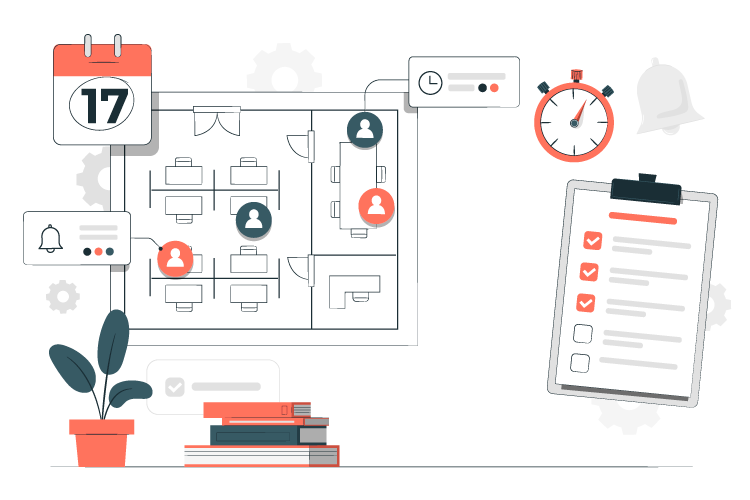
\includegraphics[width=6.5cm]{Imagens/003.ai}
		\caption{estrutura da demanda do consumidor no modelo ORANIG}
		\footnotesize
		\vspace{-0.2cm}
		\text{Fonte: adaptado de \textcite{horridge00}}
	\end{figure}
\end{frame}

\begin{frame}{Metodologia}
	\begin{itemize}
		\item \textsc{Nível de atividade} \cite{dixon82}:
		
		\begin{align*}
			\text{Leontief} \{\frac{X_{ij}}{A_{ij}}\} & = A_jZ_j
		\end{align*}
		
		onde:
		
		\begin{align*}
			\text{Leontief} \{f_i\}                   & \equiv \text{minimum} \{f_1, f_2, ..., f_r\}
		\end{align*}
	\end{itemize}
\end{frame}

\begin{frame}{Metodologia}
	\begin{itemize}
		\item \textsc{Demanda das famílias} \cite{dixon82}:
		
		\begin{align*}
			U(\bar{X}_1, ..., \bar{X}_g)
		\end{align*}
		
		sujeito a:
		
		\begin{align*}
			&\bar{X}_i = CES(X_{(is)}) \\
			&\bar{P}_{(is)}\bar{X}_{(is)} = C
		\end{align*}
	\end{itemize}
\end{frame}

\begin{frame}{Metodologia}
	\begin{itemize}
		\item No qual:
		
		\begin{align*}
			&\bar{X}_i = \frac{X_i}{A_iQ} \\
			&\bar{X}_{(is)} = \frac{X_{(is)}}{A_iA_{(is)}Q} \\
			&\bar{P}_{(is)} = P_{(is)}A_iA_{(is)}Q
		\end{align*}
	\end{itemize}
\end{frame}


\begin{frame}{Metodologia}
	\begin{itemize}[<+->]
		\item É útil para analisar impactos sobre preços relativos e variáveis macroeconômicas, focando nos ganhadores e perdedores a nível setorial \cite{anderson20, tibertietal17}.
		
		\item Entretanto, há uma restrição no modelo ao performar análises sobre distribuição de renda e pobreza:
		
		\begin{itemize}
			\item o pressuposto de Família Representativa mantém a desigualdade constante dentro de cada família;
			
			\item por isso, não capturam idealmente os efeitos de um choque sobre determinados indivíduos \textbf{dentro} de uma Família Representativa \cite{colombo08}.
		\end{itemize}
	\end{itemize}
\end{frame}

\begin{frame}{Metodologia}
	\begin{itemize}[<+->]
		\item A alternativa é através da integração com o modelo de microssimulação.
		
		\item Essa integração é particularmente útil para captar, simultaneamente, os efeitos macro e micro:
		
		\begin{itemize}
			\item efeitos diretos e indiretos do choque sobre a economia;
			\item efeito sobre as rendas e despesas a nível individual e reações frente a choques externos.
		\end{itemize}
		
		\item O modelo integrado é amplamente utilizado para avaliar impactos distributivos de choques e políticas econômicas \cite{raihan10, cicowiez16, mbanda21}.
	\end{itemize}
\end{frame}

\begin{frame}{Metodologia}
	\begin{itemize}[<+->]
		
		\item Define-se três simulações no modelo de EGC:
		
		\begin{enumerate}
			\item $\uparrow$ demanda por exportações;
			\item $\uparrow$ demanda por importações;
			\item $\uparrow$ integração regional.
		\end{enumerate}
		
		\item Opta-se pela abordagem \textit{top-down} de integração.
		
		\item O modelo de microssimulação seria composto por duas equações:
		
		\begin{enumerate}
			\item equação de renda, via correção de Heckman \cite{colombo08};
			
			\begin{align*}
				Log(YL_{mi}) = a + bX_{mi} + c \Lambda_{mi} + v_{mi}
			\end{align*}
			
			\item \textit{occupation choice model}, via logit \cite{colombo08}.
			
			\begin{align*}
				W_{mi} = \mathbbm{1}\{\alpha + \beta Z_{mi} + \gamma RW_{mi} + \epsilon_{mi} > 0\}
			\end{align*}
		\end{enumerate}
	\end{itemize}
\end{frame}

\begin{frame}{Metodologia}
	\begin{figure}
		\centering
		\includegraphics[width=14cm]{Imagens/004.ai}
		\caption{estrutura da abordagem \textit{top-down}}
		\footnotesize
		\vspace{-0.2cm}
		\text{Fonte: adaptado de \textcite{tibertietal17}}
	\end{figure}
\end{frame}


\subsection[]{Dados}

\begin{frame}{Dados}
	\begin{itemize}[<+->]
		
		\item ORANIG-BR:
		
		\begin{itemize}
			\item MCN;
			\item PNAD contínua (desagregar trabalho);
			\item POF (desagregar famílias);
			\item Comex Stat (desagregar exportações).
		\end{itemize}
		
		\item Microssimulação: dados da PNAD contínua.
	\end{itemize}
\end{frame}



% Quinta seção:
\section{Resultados esperados}

\begin{frame}{Resultados esperados}
	\begin{itemize}[<+->]
		\item Como citado anteriormente, inexiste qualquer consenso ou convergência sobre os efeitos do comércio internacional sobre desigualdade de renda e pobreza, seja entre países ou no país.
		
		\item Mesmo assim, pode-se esperar que:
		
		\begin{enumerate}
			\item pauta exportadora intensiva em recursos naturais piore os indicadores;
			
			\item já intensiva em bens manufaturados torne por melhorar os indicadores;
			
			\item aumento das exportações favoreça os indivíduos menos ricos;
			
			\item aumento das importações favoreça os indivíduos mais ricos;
			
			\item \textbf{talvez} haja redução da pobreza;
			
			\item desigualdade de renda dependerá da magnitude dos efeitos.
		\end{enumerate}
	\end{itemize}
\end{frame}



% Referências:
\bibliographpage



% Página final:
\backmatter



\end{document}


